% Please do not change the document class
\documentclass{scrartcl}

% Please do not change these packages
\usepackage[hidelinks]{hyperref}
\usepackage[none]{hyphenat}
\usepackage{setspace}
\doublespace

% You may add additional packages here
\usepackage{amsmath}
\usepackage{graphicx}
\usepackage{wrapfig}
\graphicspath{ {images/} }


% Please include a clear, concise, and descriptive title
\title{A Comparison of which Procedural Content Generator Provides More Variety and Reliability for an Indie Development Team}

% Please do not change the subtitle
\subtitle{COMP110 - Computer Architecture Essay}

% Please put your student number in the author field
\author{1507516}

\begin{document}

\maketitle

\begin{center}
\textbf{WIP - recommendation and conclusion not finished}

\end{center}


\abstract{This paper will evaluate and compare three articles; A Rhythm-Based Level Generator for 2-D platformers \cite{smith2009}, Procedural Content Generation Using Occupancy-Regulated Extension \cite{mawhorter2010} and Procedural Content Generation Using Patterns as Objectives \cite{dahlskog2014}. These articles all have their own techniques to procedurally generate content for a 2-D platformer. This article recommends that Launchpad: A Rhythm-Based Level Generator is the most appropriate Procedural Content Generator (PCG) for an indie developer that would like to implement a 2-D platformer, based on variety and extensibility.}


\section{Introduction}

The way in which we use Procedural Content Generators (PCG) to develop content for games is a vital part of the video game design process. With the recent release of popular procedurally generated 2-D games, such as \textit{Terraria}, \textit{Starbound} and \textit{Spelunky} \cite{steamtopgames}, it is important to choose a procedural content generator that suits your needs, as each is designed for a particular situation. For the context of this paper, the indie developers would like to implement a PCG onto the PC platform that can be integrated into the engine, then compile the level at runtime.

The work is motivated by the complexity and variety of all the different approaches to Procedural Content Generation, and this paper aims to provide a comparison of three different papers and make a recommendation based on the extensibility and variety of each PCG. 

The reason why these three PCG articles were chosen was because they are all designed to generate levels in the style of Super Mario Bros (SMB).
The three articles are:

Launchpad: A Rhythm-Based Level Generator for 2-D platformers \cite{smith2009} \par

Procedural Level Generation Using Occupancy-Regulated Extension \cite{mawhorter2010} \par

Procedural Content Generation Using Patterns as Objectives \cite{dahlskog2014} \par

The metrics being used to recommend the most appropriate PCG are variety and reliability. Variety can be measured by \textit{Linearity} and \textit{leniency} \footnote{leniency is how forgiving the level is to the player, e.g. levels with less obstacles or enemy's are more lenient. Linearity is a measure of the varying geometry of a level} which are metrics proposed by Smith and Whitehead \cite{smith2010}. Extensibility is being measured by how much control the developer has over the PCG and how the addition of content to the game will affect the performance of the PCG.

%Write your introduction here. A brief introduction is recommended, which should outline key details of the chosen topic and the reviewed papers, motivate the work, and provide a roadmap of key points to the reader. The motivation is quite important here, as essays should have a contribution (i.e., what is the point of the essay, and what does the reader take away from the essay) and the link between the motivation (in the introduction) and the contribution (in the conclusion) should be made clear.

\section{Review of Procedural Content Generation Articles}

\subsection{Launchpad: A Rhythm-Based Level Generator}

Launchpad generates levels out of small segments called ``\textit{rhythm groups}''  which are short, non-overlapping areas that contain a challenge for the player. I.e. a series of quick jumps or jumping back and forth between platforms. The rhythm groups are generated using a 2 tiered grammar \footnote{Grammar in this context meaning a set of rules for rewriting strings, which forms the basics of how procedural content generation works \cite{shaker2015}.} based approach.

The first stage of this creates a set of beats that correspond to a player action. This is good because it means the game can be improved by the addition of varying player actions. Furthermore each beat can be
The second stage takes the player action and creates geometry based on its parameters, this is then added to the level as a ``rhythm group''. 

To achieve guaranteed playability of levels, Launchpad takes into account a set of parameters that determine how the player moves, e.g. The maximum speed the player can move, how high they can jump etc \cite{smith2012web}. This means that each level that is generated does not create sections that the player cannot pass. Furthermore designers can have a lot more control over the design of player movement without having to be concerned with level geometry, thus also increasing the extensibility of the PCG.


However, this approach is designed for a ``speedrun''  type of gameplay, where player dexterity is key \cite{smith2009}. This means that it does not currently work well with different types of gameplay, i.e. exploration.


\subsection{Procedural Level Generation Using Occupancy-Regulated Extension}

This procedural level generator is able to generate levels without knowing anything about how the game works. This method works by using a library of chunks and assembling them based on a complex set of parameters. 

This algorithm generates the content in 3 stages, firstly it selects the location at which to start generating geometry. It then selects chunks from the library that is then tested with its filtering and selection algorithms to see if it is appropriate to place at that location. Lastly, that chunk is integrated within the existing content.

Compared to Launchpad, this method requires a large amount of human authored content to be available in order to get a varied level. Furthermore, this method is not very extensible as the more items are added to the library the longer it takes to generate a level. Even after the level is generated, it still requires a large amount of post-processing to make the game playable.

However when done correctly with the right settings, this approach can generate some very creative and complex levels as seen in figure 1 .

This approach does not guarantee playable levels, which is a very undesirable property when creating a level.



\subsection{Procedural Content Generation Using Patterns as Objectives}

Dahlskog and Togelius take an interesting approach to PCG, by looking for patterns in the way levels are structured in an original game such as SMB, then analyzing that level design to generate levels that use the same level design techniques. This means that the levels can maintain a high quality, but still be varied at the same time.

This method works by identifying ``micro-patterns'' and ``meso-patterns'' in an existing game, such as SMB. Micro-patterns are a vertical 1-block wide slice of the level, and meso-patterns are the way in which micro-patterns are arranged. The generator then uses the micro-patterns as building blocks to generate a new level.

However this PCG is not ideal for an indie developer as the implementation requires a version of an existing game to work, this means that the developer must create a game and a well designed level in order to generate more levels of the same type. Furthermore it does not allow for much linearity if it is being based of a level without a varied level.






%Write the main body of your essay here. Add more sections if appropriate. You may choose to write about each of your three papers in its own section, or you may choose a different structure. Either way, remember that you are being assessed on technical insight and analysis: it is not enough to merely summarise the contents of the three papers. You must demonstrate the ability to make inferences beyond what is written in the papers, and to draw the three papers together into a single coherent narrative.

\section{Recommendation}

Figure \ref{fig:PCG} shows a set of images displaying the different outputs of each PCG.
%\includegraphics[width=\textwidth][h]{archtecture-images}


\begin{figure}[h]
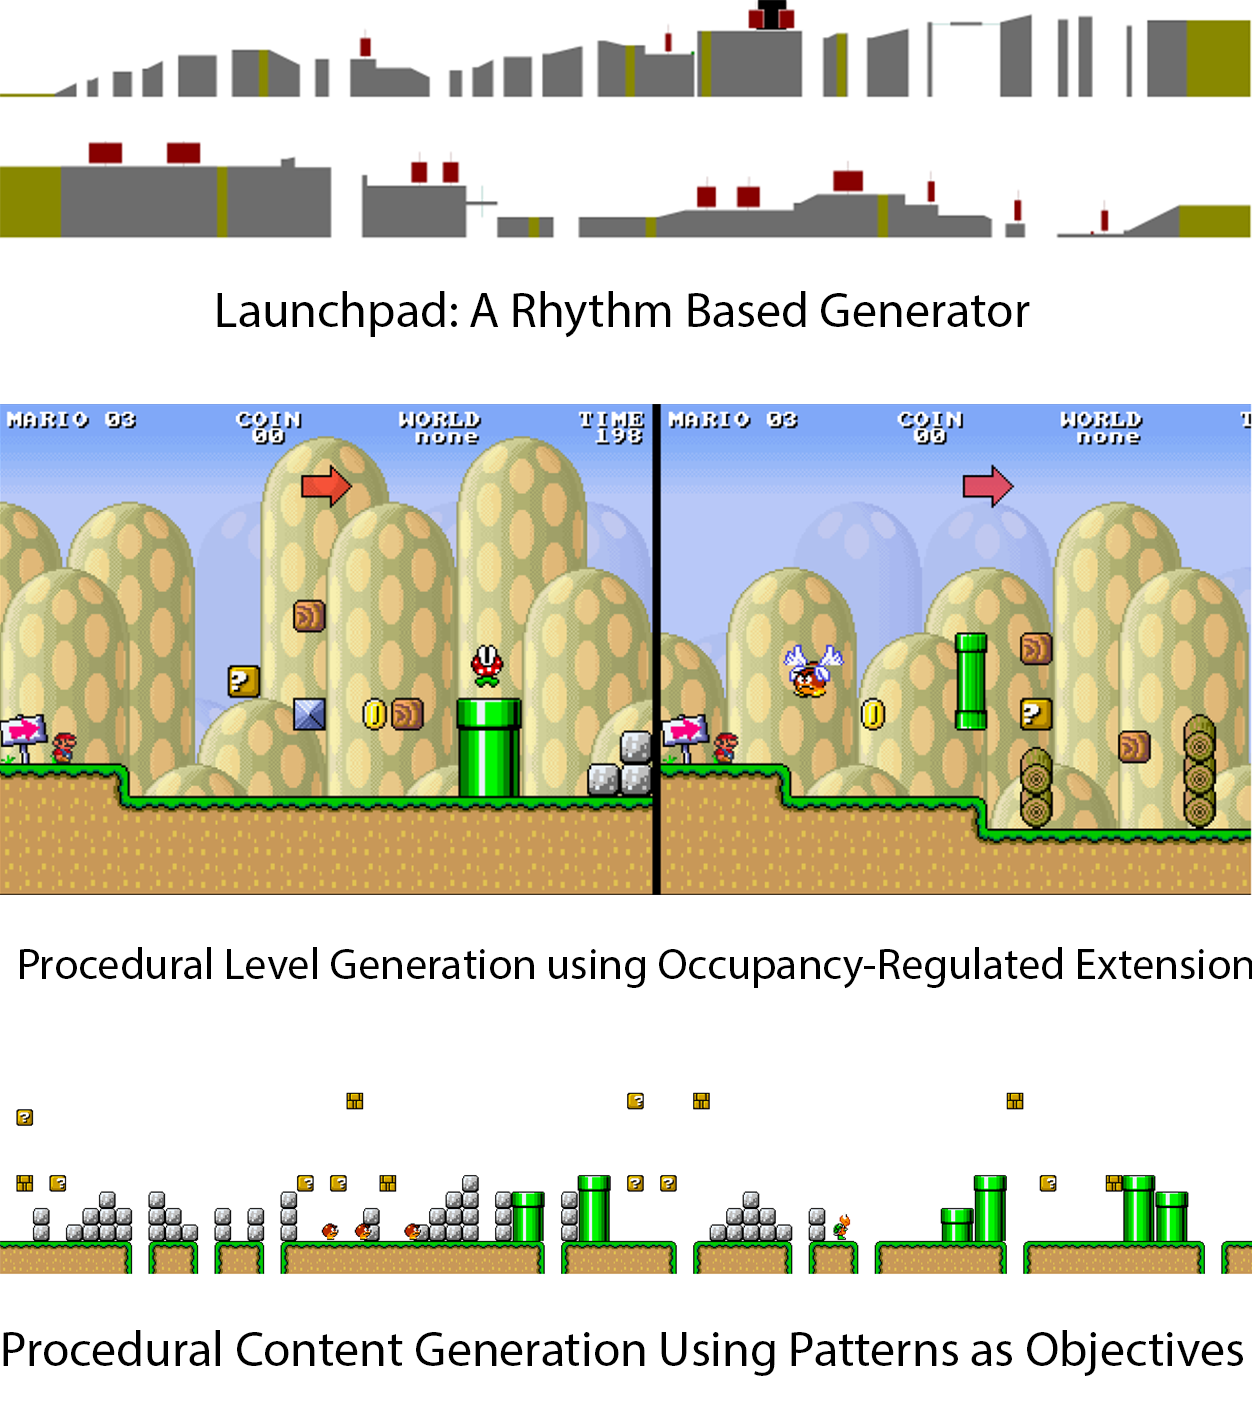
\includegraphics[width=8cm]{archtecture-images}
    \caption{PCG level comparison}
    \label{fig:PCG}
\end{figure}



%\begin{wrapfigure}[h]{r}{0.75\textwidth} %this figure will be at the right
%   \centering
 %   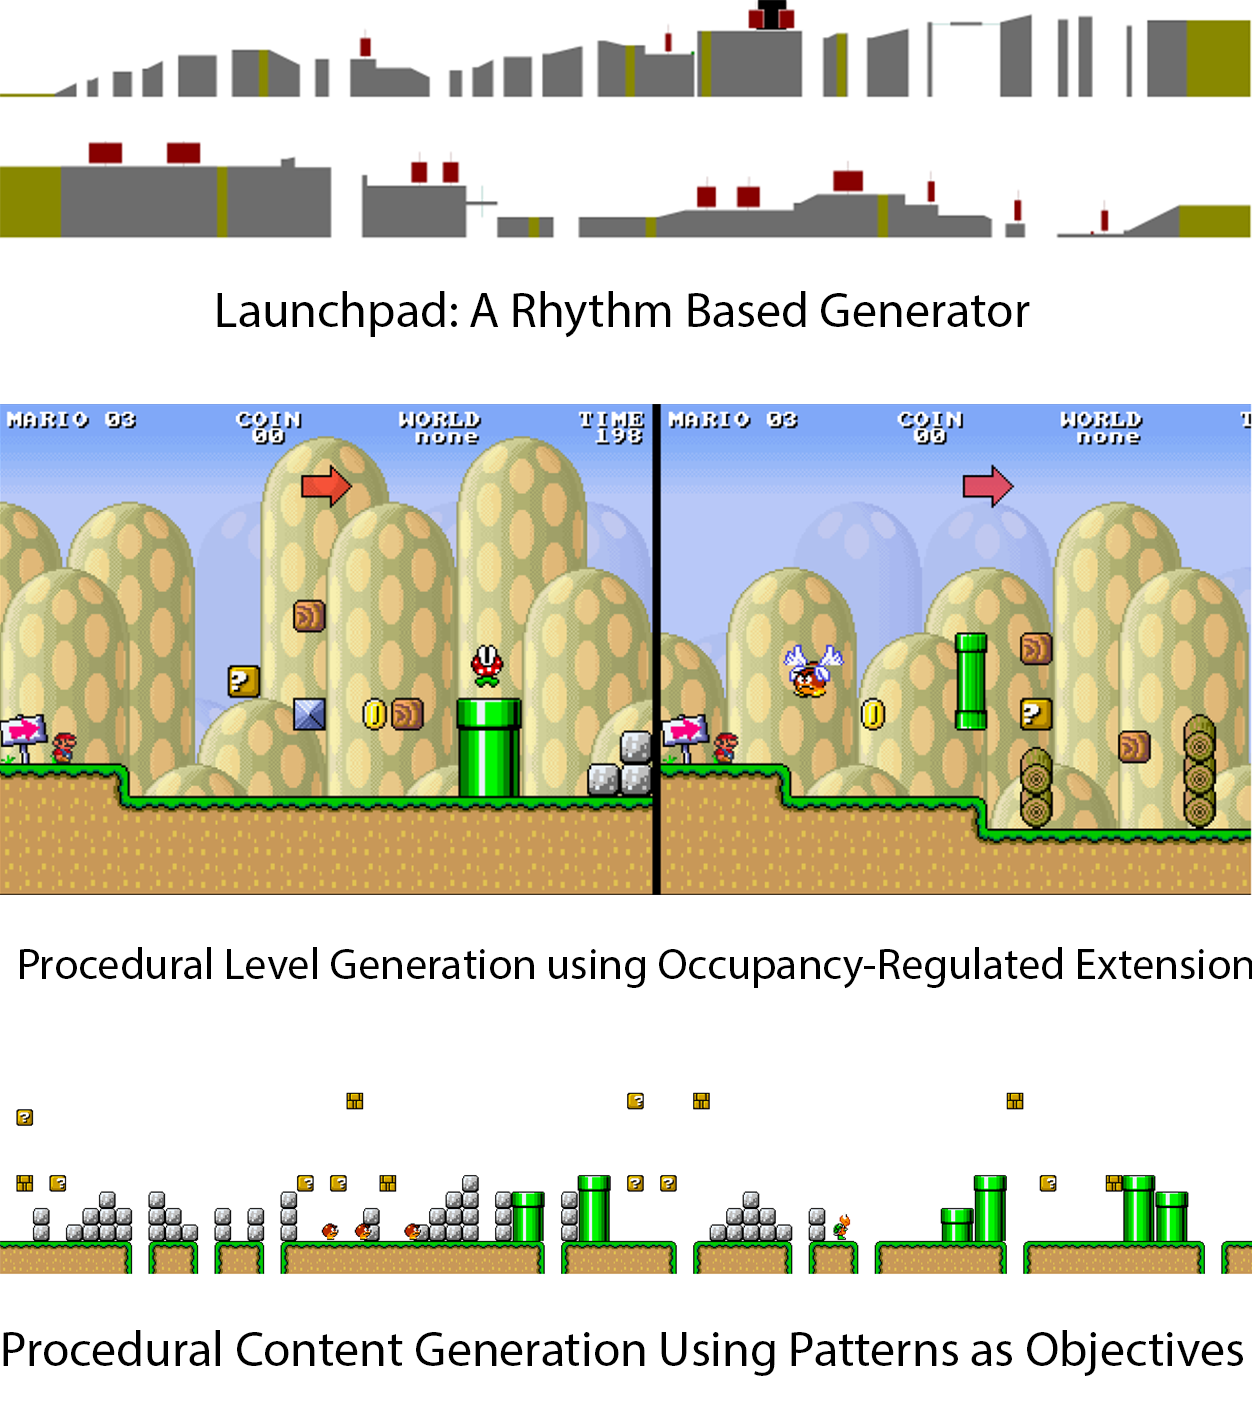
\includegraphics[width=0.5\textwidth]{archtecture-images}
 %   \caption{PCG level comparison}
 %   \label{fig:PCG}
%\end{wrapfigure}



%Your essay must make a clear recommendation, in terms of which of the three techniques you have reviewed is the best according to whichever metric or metrics you feel is most appropriate. You must justify your choice, backing it up with empirical evidence. However remember that an academic essay is not a murder mystery: you should already have briefly discussed your recommendation in the introduction and in other parts of the essay. Do not save it for a grand reveal at the end.

\section{Conclusion}

Write your conclusion here. The conclusion should do more than summarise the essay, making clear the contribution of the work and highlighting key points, limitations, and outstanding questions. It should not introduce any new content or information.

\bibliographystyle{ieeetran}
\bibliography{comp110_architecture}

\end{document}
